\chapter{Evaluations}
\label{chap-five}

\section{Methodology}
We have used leave-one cross testing for all experimentations. Most data sets for experimentation are stock databases available on the UCI machine-learning repository while some source data sets are Microsoft released source data sets for machine learning.
These data sources are then divided into data sets. Depending on the size of the data source\cite{uci_machine_repo} we may have any where between 10 to 43 data sets, where in all save one are treated as historic data sets. We have also allowed all algorithms to converge to the same epsilon error rate thus ensuring the run time comparison for similar quality output for algorithms.
All experiments have been carried out on Octa core Intel Xeon CPU E5-2650 Running Ubuntu Linux 14.04 LTS with 16GB of RAM.
\section{Experiments}
To demonstrate the efficacy and efficiency of our program we evaluate our approach by testing it on various large real world data-sets and compare our algorithm to two most frequently used and vastly accepted K-Means initialization algorithms: standard K-Means (Random Select initialization also known as Lloyd's Algorithm) and K-Means++ initialization (Weighed Probability based initialization based on squared of distance from initial randomly selected center). Both the above algorithms are implemented in the OpenCV library, which has been used as the standard library for Lloyd’s Algorithm implementation. We run all three algorithms on the same data sets with the same error rate for convergence.
We have also compared the historical data-set selected by our algorithm to all other data-sets available in history to show the accuracy of our algorithm in selecting the best available data-set.

\begin{figure}[h!]
    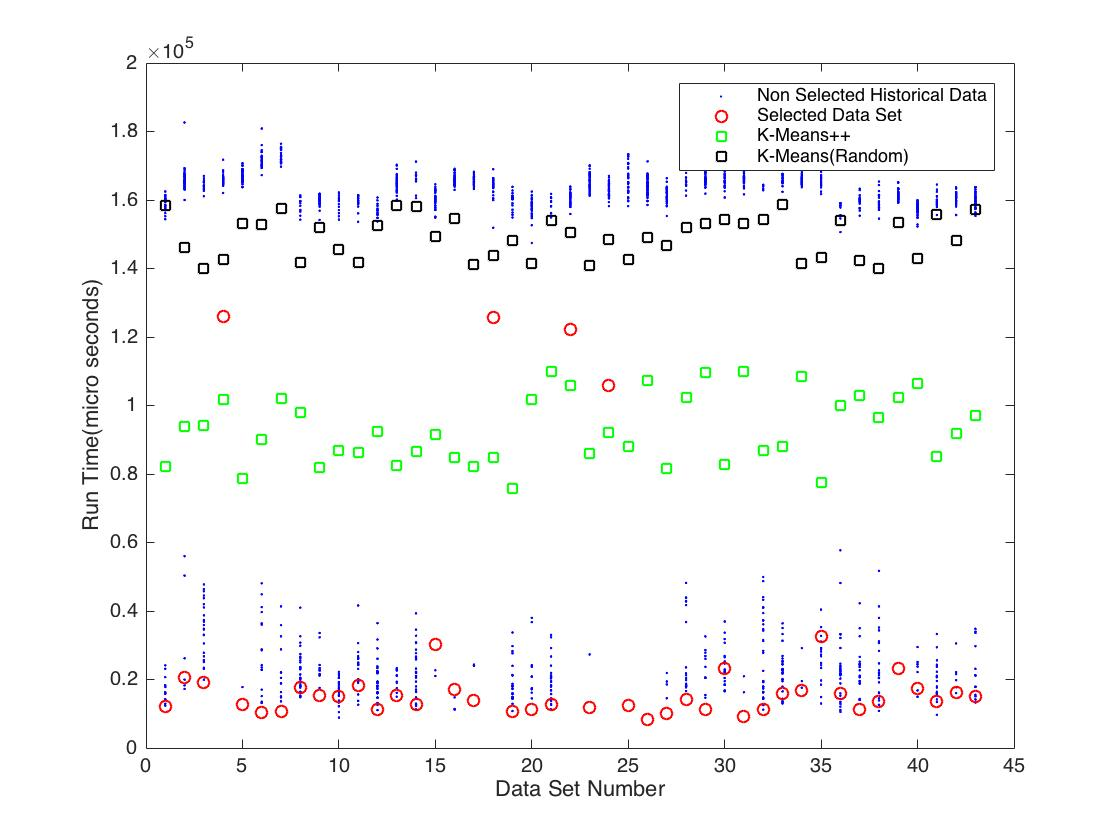
\includegraphics[width=\textwidth]{Chapter-5/figs/road_240}
    \caption{Hit-Rate (Road Network k=120)}
    \centering
    \label{fig:gas_240_selection}
\end{figure}

\begin{figure}[t!]
    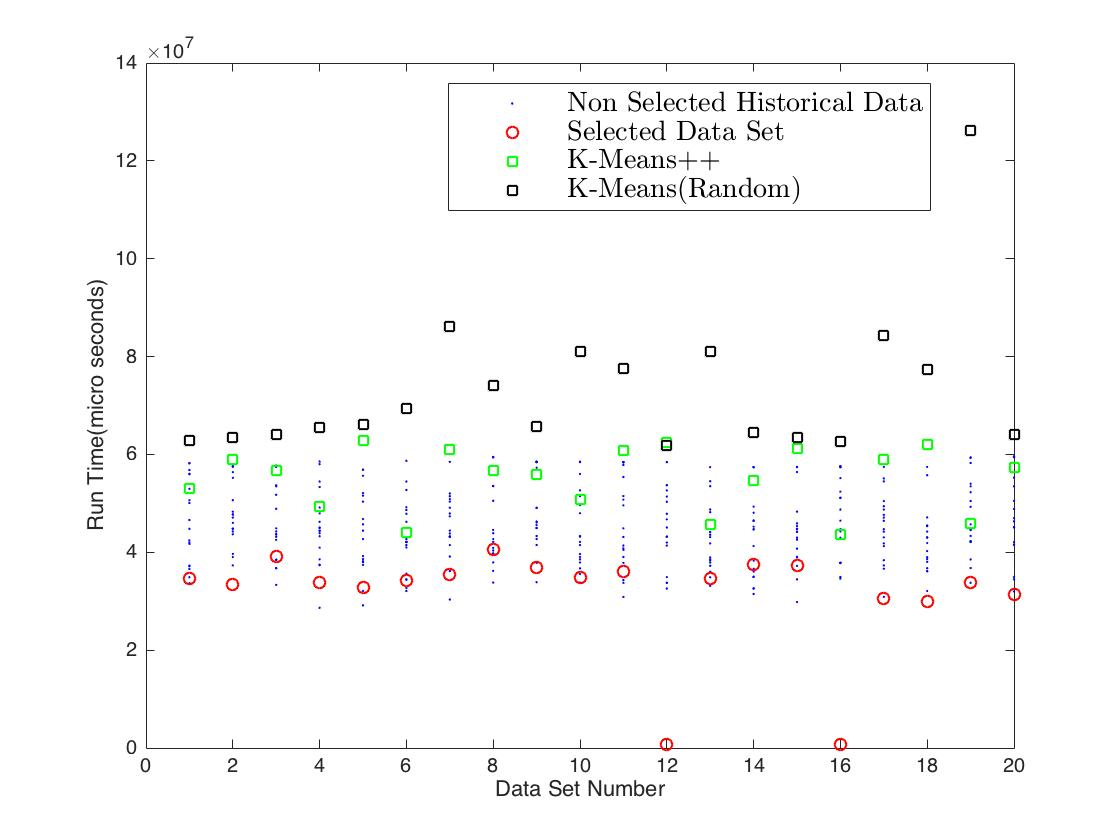
\includegraphics[width=\textwidth]{Chapter-5/figs/nnData_600}
    \caption{Hit-Rate (Caltec 101 for k=600)}
    \centering
    \label{fig:caltec_600_selection}
\end{figure}

\setlength{\arrayrulewidth}{0.2mm}
\setlength{\tabcolsep}{10pt}
%\renewcommand{\arraystretch}{1}
\begin{table*}[h!]
% \begin{minipage}{\textwidth}
\centering
% \begin{center}
\begin{tabular}{|l|c|c|c|r|}
\hline\hline
    \textbf{Data-set Name} & \textbf{History Data-set cnt.} & \textbf{Cluster Count} & \textbf{Top 5 cnt} & \textbf{Hit Rate \%} \\
\hline\hline
    \textbf{Road Network}   & 43 &
    \begin{tabular}{c} 40 \\ 80 \\ 120 \\ 240 \end{tabular} &
    \begin{tabular}{c} 42 \\ 41 \\ 43 \\ 43 \end{tabular} &
    \begin{tabular}{c} 97.67\% \\ 95.34\% \\ 100\% \\ 100\% \end{tabular} \\
\hline
    \textbf{Kegg Network}   & 10 &
    \begin{tabular}{c} 40 \\ 80 \\ 120 \\ 240 \end{tabular} &
    \begin{tabular}{c} 8 \\ 9 \\ 8 \\ 8 \end{tabular} &
    \begin{tabular}{c} 80\% \\ 90\% \\ 80\% \\ 80\% \end{tabular} \\
\hline
    \textbf{US Gas Sensor Data}   & 36 &
    \begin{tabular}{c} 40 \\ 80 \\ 120 \\ 240 \end{tabular} &
    \begin{tabular}{c} 28 \\ 29 \\ 29 \\ 28 \end{tabular} &
    \begin{tabular}{c} 77.7\% \\ 80.5\% \\ 80.5\% \\ 77.7\% \end{tabular} \\
\hline
    \textbf{NotreDame}   & 20 &
    \begin{tabular}{c} 40 \\ 80 \\ 120 \\ 240 \end{tabular} &
    \begin{tabular}{c} 17 \\ 18 \\ 17 \\ 17 \end{tabular} &
    \begin{tabular}{c} 85\% \\ 90\% \\ 85\% \\ 85\% \end{tabular} \\
\hline
    \textbf{Tiny}   & 20 &
    \begin{tabular}{c} 80 \\ 120 \\ 240 \\ 360 \\ 480 \\ 600 \end{tabular} &
    \begin{tabular}{c} 20 \\ 18 \\ 16 \\ 17 \\ 18 \\ 18 \end{tabular} &
    \begin{tabular}{c} 100\% \\ 90\% \\ 80\% \\ 85\% \\ 90\% \\ 90\% \end{tabular} \\
\hline
    \textbf{Uk Bench}   & 20 &
    \begin{tabular}{c} 80 \\ 120 \\ 240 \\ 360 \\ 480 \\ 600 \end{tabular} &
    \begin{tabular}{c} 20 \\ 18 \\ 16 \\ 17 \\ 18 \\ 18 \end{tabular} &
    \begin{tabular}{c} 100\% \\ 90\% \\ 80\% \\ 85\% \\ 90\% \\ 90\% \end{tabular} \\
\hline
    \textbf{Caltec 101}   & 20 &
    \begin{tabular}{c} 80 \\ 120 \\ 240 \\ 360 \\ 480 \\ 600 \end{tabular} &
    \begin{tabular}{c} 20 \\ 18 \\ 16 \\ 17 \\ 18 \\ 18 \end{tabular} &
    \begin{tabular}{c} 100\% \\ 90\% \\ 80\% \\ 85\% \\ 90\% \\ 90\% \end{tabular} \\
\hline
\end{tabular}
\caption{Selection Hit Rate K-Means History Reuse}
\label{table:1}
% \end{center}
\end{table*}

\textbf{Consistent Selection of Best Match Historical Data-set from History:} The experiments run, show that our algorithm is able to consistently able to select one of the top 5 data-sets for history reuse from available historical data-sets. By consistent, we mean that our algorithm is able to select one of the top 5 available data sets with hit rate of above seventy percent across data sets irrespective of the size and the cluster count. This is expected as we aim to compare data set based on similarity while the cluster count is not taken into consideration in the matching process. \textbf{\textit{Table \ref{table:1}}} shows the hit rate for our algorithm.
We can clearly see from the table that our algorithm is able to select one of the top 5 best data sets for historical reuse from the available data sets consistently irrespective of the cluster count and the total historically available data sets. 
This thus validates our theory for probabilistic selection for matching data sets using the \textbf{Welch's Test} for null hypothesis testing for similarity of data sets. We are also able to see clearly that our selection criteria continues to perform well across a wide range of cluster counts and thus validates our hypothesis that data-set similarity should be used as the primary measure to gauge quality of data-set for history reuse without the explicit need for taking into account the total number of clusters \textit{(k)} the data-set is to be clustered into. We have chosen to limit the total number of clusters to 256 so as to have meaningful clusters for data sets of relatively small sizes.
Columns 3, 4 and 5 show us how well our data-set selection algorithm works across various cluster indexes and also how little variation is seen in the performance of the data-sets selected by our algorithm irrespective of the number of clusters \textit{(k)}. We also show that our hit rate is a minimum of 70 percent (Some error is to be expected as the selection algorithm works on probabilistic model for making best guess.)
Figures \ref{fig:gas_240_selection} and \ref{fig:caltec_600_selection} show how our selected historical data set performs in comparison to all other data sets available for selection in our history database. We  see from them, the accuracy of algorithm in consistently choosing one of the best match data sets from history with high accuracy (>~ 75\%). We see that our algorithm chooses either the best match data set or data set close to best match. This proves the accuracy of our algorithm.
\textbf{Consistent Scalable approach to Selection:} Our experiments also show that our method scales well with the increase in dimensionality of data \textit{(d)}, the size of the data-set\textit{(n)} and the cluster count\textit{(k)}. \textbf{\textit{Figures \ref{fig:selection_overhead} and \ref{fig:selection_overhead_large}}} show our experimental results for various data sets with varying dimensionality and sizes. These figures clearly show that for any given data set the selection time is completely independent of the cluster count \textit{(k)}. This is in complete contrast to both the  \textit{random K-Means (Lloyd's Algorithm)} and the K-Means++ algorithm where the initialization overhead is directly proportional to the cluster count \textit{(k)} for the data set. Our experimental results also serve the purpose of showing us that our initialization methodology has an over head very small compared to the total run time of the algorithm even for the smallest of chosen cluster counts. This combined with the proven choosing of better initialization centroids (as seen in Table \ref{table:total_runtime_comparison} and Table \ref{table:iteration_comparison} which show an overall improvement in both run time as well as the number of iterations taken for the data to converge) gives us a win-win situation of a comprehensively better initialization methodology in comparison to both the previously mentioned methods.


\begin{figure}[t!]
    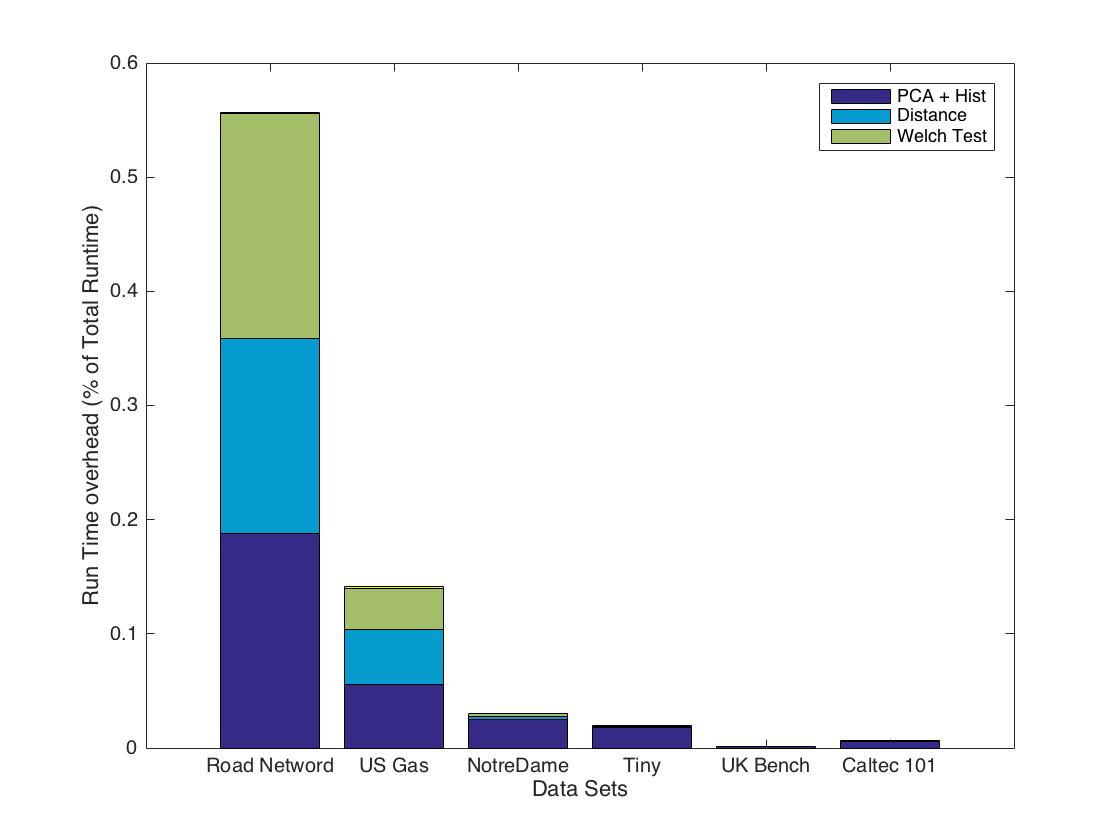
\includegraphics[width=\textwidth]{Chapter-5/figs/stacked_overhead}
    \caption{Best Match Selection Overhead (Maximum for Small \textit{k})}
    \centering
    \label{fig:selection_overhead}
\end{figure}

\begin{figure}[t!]
    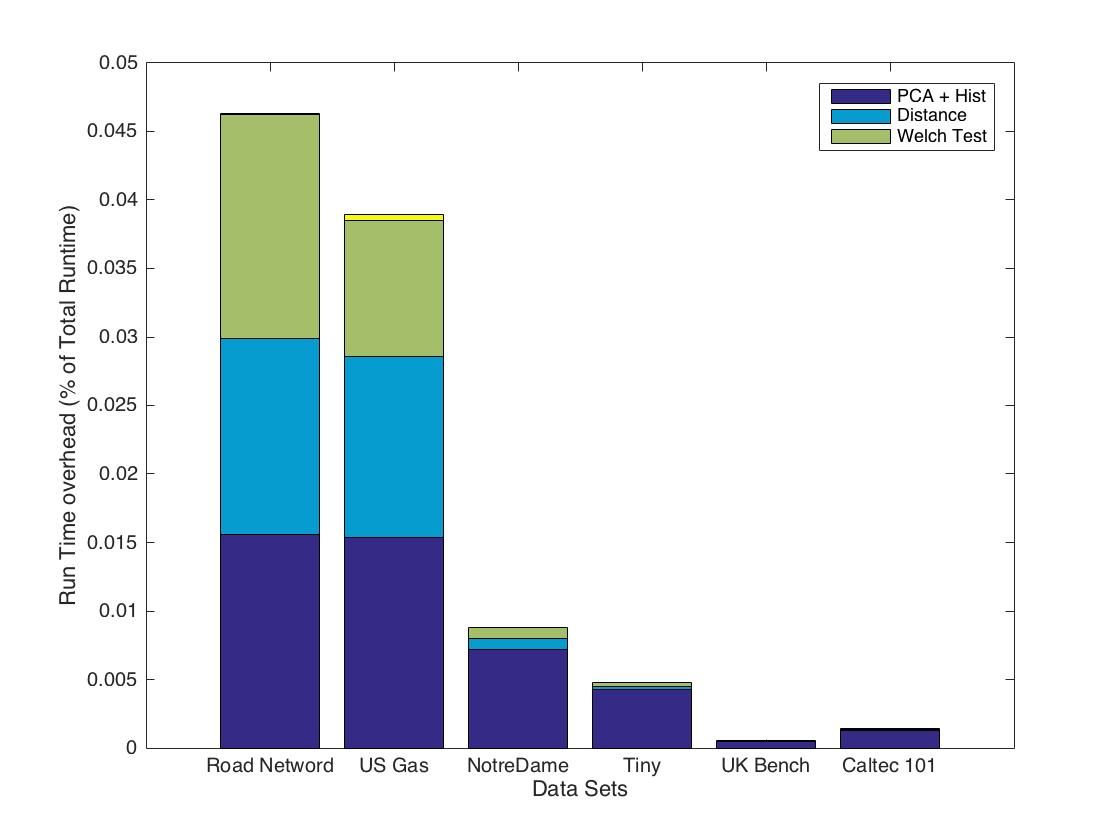
\includegraphics[width=\textwidth]{Chapter-5/figs/stacked_overhead_large}
    \caption{Best Match Selection Overhead (Minimum for Large \textit{k})}
    \centering
    \label{fig:selection_overhead_large}
\end{figure}

\begin{figure}[t!]
    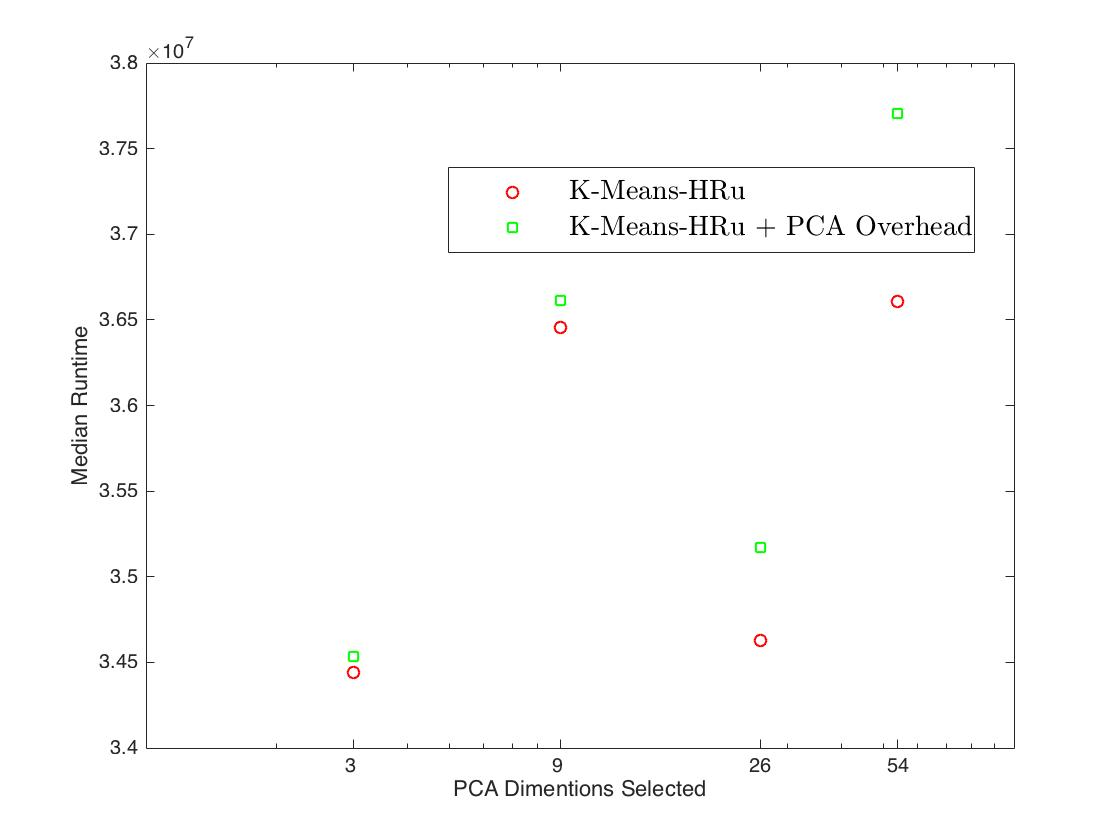
\includegraphics[width=\textwidth]{Chapter-5/figs/PCA_results}
    \caption{Performance for various PCA Dimension Count(Caltec 101; K = 600). Default PCA Dims: 3}
    \centering
    \label{fig:pca_overhead}
\end{figure}

Referencing the above mentioned tables and figures, we can also see that our selection mechanism takes only a very small percentage of the total run time for the algorithm for larger data sets (<~0.1\%) and while it may be a significant part of the initialization for smaller data sets the quality improvement in the initialization centroids is sufficient to offset the run time for the algorithm to be a viable initialization methodology for all data sets of varying sizes. 
Though speed up using our methodology is seen in all cases, it is best suited for larger data sets, as in that case our overhead for history best match selection almost becomes negligible.

From \textit{\textbf{Figure \ref{fig:pca_overhead}}} we can also see that even while retaining higher variances for historic data sets, no further speedup is seen in run time while the introduced overhead becomes a significant percentage for the total run time and may lead to further overheads as data set sizes increase.

\bgroup
\setlength{\arrayrulewidth}{0.2mm}
\setlength{\tabcolsep}{10pt}
\renewcommand{\arraystretch}{1}
\begin{table*}[t!]
\begin{minipage}{\textwidth}
\centering
%\begin{top}
\begin{tabular}{|l|c|c|c|c|c|c|r|}
\hline\hline
    \textbf{Data-set} & \textbf{n} & \textbf{d} & \textbf{k} & \textbf{K-Means (Time $\mu$S)} & \textbf{K-Means++} & \textbf{K-Means-HRU}\\
\hline\hline
    \textbf{Road Net.}   & 1.0E4 & 3 &
    \begin{tabular}{c} 40 \\ 80 \\ 120 \\ 240 \end{tabular} &
    \begin{tabular}{c} 8.5E4 \\ 1.6E5 \\ 2.01E5\\ 2.4E5\\ \end{tabular}&
    \begin{tabular}{c} 1.7X \\ 2.4X \\ 2.2X \\ 1.8X \\ \end{tabular} &
    \begin{tabular}{c} 6.7X \\ 10.0X \\ 10.0X \\1.6X \\ \end{tabular}\\
\hline
    \textbf{Kegg Net.}   & 2.0E4 & 10 &
    \begin{tabular}{c} 40 \\ 80 \\ 120 \\ 240 \end{tabular} &
    \begin{tabular}{c} 1.9E5 \\ 2.8E6 \\ 3.9E5 \\ 6.3E5 \\ \end{tabular} &
    \begin{tabular}{c}  2.5X \\ 1.9X \\ 1.6X \\ 1.9X \\ \end{tabular}&
    \begin{tabular}{c} 2X \\ 2.2X \\  2.8X \\ 3.2X \\ \end{tabular}\\
\hline
    \textbf{US Gas}   & 1.45E4 & 13 &
    \begin{tabular}{c} 40 \\ 80 \\ 120 \\ 240 \end{tabular} &
    \begin{tabular}{c} 3.2E5 \\ 4.7E5 \\ 5.2E5 \\ 8.9E5 \end{tabular} &
    \begin{tabular}{c} 2.4X \\ 1.9X \\ 1.9X \\ 1.7X \\  \end{tabular}&
    \begin{tabular}{c} 5.6X \\ 4.4X \\ 3.9X \\ 4.3X \\ \end{tabular}\\
\hline
    \textbf{NotreDame}   & 1.45E4 & 13 &
    \begin{tabular}{c} 40 \\ 80 \\ 120 \\ 240 \\ \end{tabular} &
    \begin{tabular}{c} 2.1E6 \\ 3.8E6 \\ 5.5E6 \\ 1.02E6\\ \end{tabular} &
    \begin{tabular}{c} 1.2X \\ 1.3X \\ 1.3X \\ 1.4X \\ \end{tabular}&
    \begin{tabular}{c} 2.4X \\ 2.3X \\ 2.3X \\ 2.3X \\ \end{tabular}\\
\hline
    \textbf{Tiny}   & 1.45E4 & 13 &
    \begin{tabular}{c} 80 \\ 120 \\ 240 \\ 360 \\ 480 \\ 600 \end{tabular} &
    \begin{tabular}{c} 0.9E8 \\ 1.3E8 \\ 2.5E8 \\ 3.2E8 \\ 3.9E8 \\ 4.3E8 \\ \end{tabular} &
    \begin{tabular}{c} 1.4X \\ 1.6X \\ 2.1X \\ 2.0X \\ 2.9X \\ 2.9X \\ \end{tabular}&
    \begin{tabular}{c} 2.8X \\ 2.9X \\ 3.8X \\ 2.7X \\ 4.1X \\ 4.1X \\  \end{tabular}\\
\hline
    \textbf{Uk Bench}   & 1.45E4 & 13 &
    \begin{tabular}{c} 80 \\ 120 \\ 240 \\ 360 \\ 480 \\ 600 \end{tabular} &
    \begin{tabular}{c} 1.7E7 \\ 2.3E7 \\ 4.2E7 \\ 4.7E7 \\ 5.8E7 \\ 6.8E7 \\ \end{tabular} &
    \begin{tabular}{c} 1.1X \\ 1.2X \\ 1.4X \\ 1.25X \\ 1.4X \\ 1.3X \\ \end{tabular}&
    \begin{tabular}{c} 2.7X \\ 2.5X \\ 2.5X \\ 2.4X \\ 2.1X \\ 2.3X \\ \end{tabular}\\
    
\hline
    \textbf{Caltec 101}   & 1.45E4 & 13 &
    \begin{tabular}{c} 80 \\ 120 \\ 240 \\ 360 \\ 480 \\ 600 \end{tabular} &
    \begin{tabular}{c} 1.9E7 \\ 2.2E7 \\ 4.2E7 \\ 5.3E7 \\ 6.5E7 \\ 7.3E7 \\ \end{tabular} &
    \begin{tabular}{c} 1.2X \\ 1.1X \\  1.4X \\ 1.4X \\   1.3X \\ 1.3X \\ \end{tabular}&
    \begin{tabular}{c} 2.6X \\ 2.1X \\ 2.3X \\ 2.3X \\ 2.2X \\ 2.1X \\ \end{tabular}\\
\hline
\end{tabular}
\caption{Runtime comparison: K-Means, K-Means++ and K-Means-HRU \textit{(*All times in $\mu$S)}}
\label{table:total_runtime_comparison}
%\end{top}
\end{minipage}
\end{table*}
\egroup

\textbf{Consistent Speed up for K-Means algorithm:} The end requirement of any initialization algorithm is to ensure that we achieve a consistent speed up over previous approaches. While running our initialization algorithm for K-Means we were able to see consistent speed up in run-time of algorithm as compared to both K-Means and K-Means++ algorithm for all data sets across a wide range of cluster counts ranging from 40 to 600. This is though dependent on quality of historical data sets available. A bad match may lead to relatively bad starting points which in turn leads to an increase in time taken for convergence. Not withstanding the above argument we were able to see consistently good performance by our algorithm for real data sets. This is largely due to the normalization of the data sets using the PCA based approach and then using cluster information based on this normalized data rather than the actual data. This also removes the need for the data to have Gaussian distribution. This gives a higher chance of finding a better historical match, thus giving consistent speed up over various data sets with different dimensionality\textit{(d)} and different cardinality\textit{(n)} for varying cluster counts \textit{k}.

Figures \ref{fig:box_speedup_small} and \ref{fig:box_speedup_large} shows the range of speed up across various data sets with varying degrees of freedom as well as different dimensionality for the same cluster counts. We can clearly see from the graphs that our algorithm consistently outperforms both the \textit{random K-Means(Lloyd’s Algorithm)} and the \textit{K-Means++ algorithm} in run time performance.


\begin{figure*}[p!]
    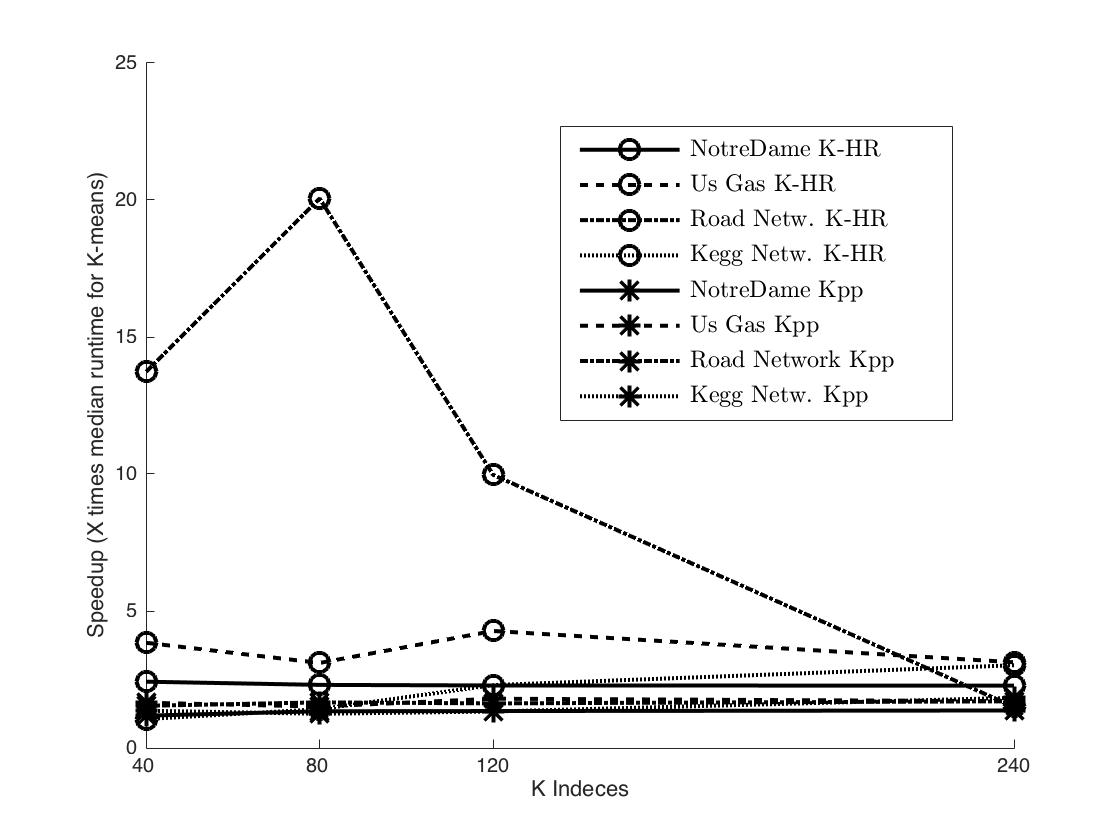
\includegraphics[width=\textwidth, height = 0.7\textheight, scale=1]{Chapter-5/figs/k_means_speedup_line_small}
    \caption{Median Speed up, Small Data (k=240)}
    \centering
    \label{fig:line_speedup_small}
\end{figure*}

\begin{figure*}[h!]
    \centering
        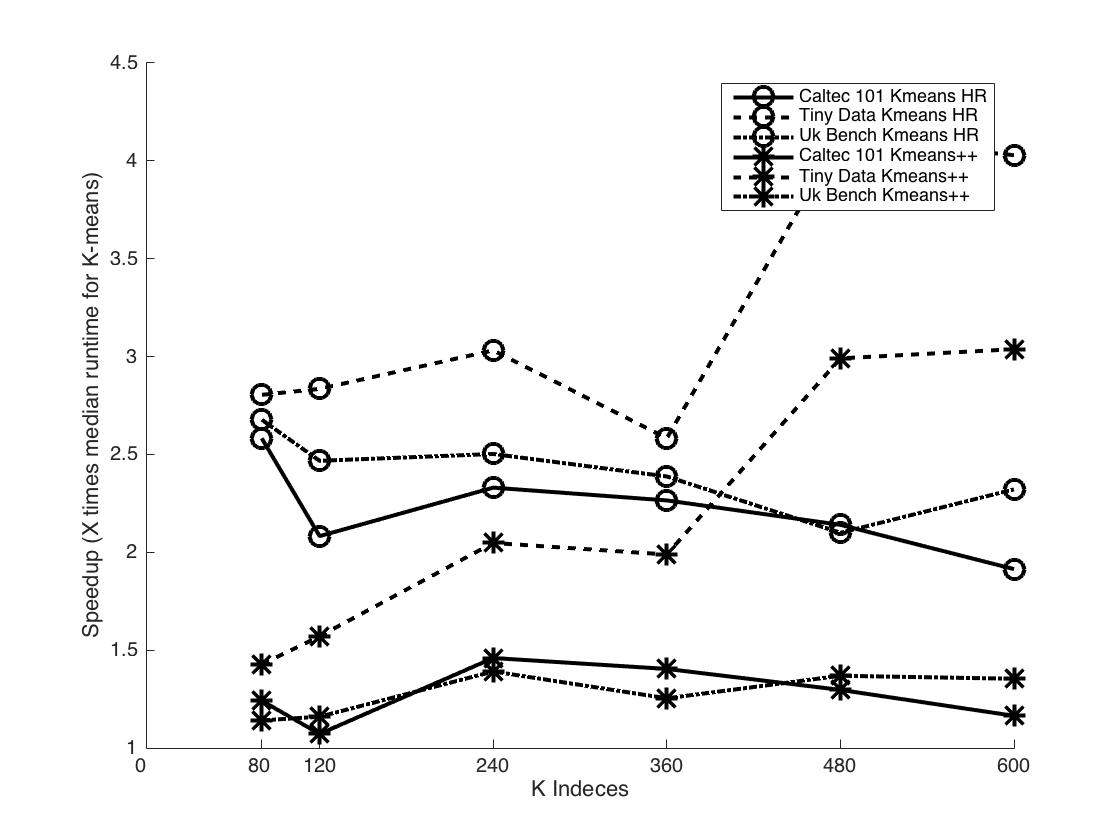
\includegraphics[width=\textwidth, height = 0.5\textheight, scale=1]{Chapter-5/figs/k_means_speedup_line_large}
    \caption{Median Speed up, Large Data (k=600)}
    \label{fig:line_speedup_large}
\end{figure*}

Figures \ref{fig:line_speedup_small} and \ref{fig:line_speedup_large} depict the speed up seen by our algorithm over various cluster sizes for all data sets. We can see that the general trend is that speed up seen is in general higher for larger cluster count. This is particularly true because as the cluster count increases we see a speed up in both the initialization method as well as the actual run time because of the improvement seen in the initialization centroids.

\setlength{\arrayrulewidth}{0.2mm}
\setlength{\tabcolsep}{10pt}
\renewcommand{\arraystretch}{1}
\begin{table*}[t!]
\begin{minipage}{\textwidth}
\centering
%\begin{top}
\begin{tabular}{|l|c|c|c|c|c|c|r|}
\hline\hline
    \textbf{Data-set} & \textbf{n} & \textbf{d} & \textbf{k} & \textbf{K-Means (Random)} & \textbf{K-Means++} & \textbf{K-Means-HRu}\\
\hline\hline
    \textbf{Road Net.}   & 1.0E4 & 3 &
    \begin{tabular}{c} 40 \\ 80 \\ 120 \\ 240 \end{tabular} &
    \begin{tabular}{c} 128 \\ 119 \\ 110 \\ 102 \\ \end{tabular}&
    \begin{tabular}{c} 69 \\ 52 \\ 46 \\ 79 \\ \end{tabular} &
    \begin{tabular}{c} 39 \\ 27 \\ 30 \\ 82 \\ \end{tabular}\\
\hline
    \textbf{US Gas}   & 1.45E4 & 13 &
    \begin{tabular}{c} 40 \\ 80 \\ 120 \\ 240 \end{tabular} &
    \begin{tabular}{c} 117 \\ 111 \\ 106 \\ 100 \\ \end{tabular} &
    \begin{tabular}{c} 58 \\ 59 \\ 58 \\ 55 \\ \end{tabular}&
    \begin{tabular}{c} 26 \\ 32 \\ 33 \\ 37\\ \end{tabular}\\
\hline
    \textbf{NotreDame}   & 1.45E4 & 13 &
    \begin{tabular}{c} 40 \\ 80 \\ 120 \\ 240 \\ \end{tabular} &
    \begin{tabular}{c} 162 \\ 154 \\ 132 \\ 103 \\ \end{tabular} &
    \begin{tabular}{c} 142 \\ 114.5 \\ 101 \\ 74 \\ \end{tabular}&
    \begin{tabular}{c} 69.5 \\ 65 \\ 60 \\ 48.5 \\ \end{tabular}\\
\hline
    \textbf{Tiny}   & 1.45E4 & 13 &
    \begin{tabular}{c} 80 \\ 120 \\ 240 \\ 360 \\ 480 \\ 600 \end{tabular} &
    \begin{tabular}{c} 195 \\ 181.5 \\ 168.5 \\ 129.5 \\ 119.5 \\ 111.5 \\ \end{tabular} &
    \begin{tabular}{c} 164 \\ 154.5 \\ 120.5 \\ 99.5 \\ 87.5 \\ 72 \\ \end{tabular}&
    \begin{tabular}{c} 108 \\ 98 \\ 87.5 \\ 74 \\ 67 \\ 58 \\ \end{tabular}\\
\hline
    \textbf{Uk Bench}   & 1.45E4 & 13 &
    \begin{tabular}{c} 80 \\ 120 \\ 240 \\ 360 \\ 480 \\ 600 \end{tabular} &
    \begin{tabular}{c} 274.5 \\ 273.5 \\ 251 \\ 233 \\ 216 \\ 196 \\ \end{tabular} &
    \begin{tabular}{c} 191 \\ 174.5 \\ 121 \\ 102 \\ 79.5 \\ 72 \\ \end{tabular}&
    \begin{tabular}{c} 85.5 \\ 82 \\ 75 \\ 70.5 \\ 63.5 \\ 57.5 \\ \end{tabular}\\
    
\hline
    \textbf{Caltec 101}   & 1.45E4 & 13 &
    \begin{tabular}{c} 80 \\ 120 \\ 240 \\ 360 \\ 480 \\ 600 \end{tabular} &
    \begin{tabular}{c} 219.5 \\ 171 \\ 178 \\ 146.5 \\ 137 \\ 108 \\ \end{tabular} &
    \begin{tabular}{c} 175.5 \\ 156.5 \\ 116.5 \\ 100 \\ 90 \\ 79 \\ \end{tabular}&
    \begin{tabular}{c} 84.5 \\ 80.5 \\ 74 \\ 69 \\ 61 \\ 58.5 \\ \end{tabular}\\
\hline
\end{tabular}
\caption{Median Iteration count comparison for K-Means, K-Means++ and K-Means with History Reuse.}
\label{table:iteration_comparison}
%\end{top}
\end{minipage}
\end{table*}

Results seen in Figures \ref{fig:selection_overhead} and \ref{fig:selection_overhead_large}  and Table \ref{table:total_runtime_comparison} together also show us that the speed ups are consistent irrespective of the cluster counts \textit{(k)} in terms of both the run time of the algorithms and the number of iterations taken for the convergence of the algorithm to similar error rate. This is again an intuitive results which confirms our hypothesis: a consistent selection methodology independent of the cluster index size would lead to sizable improvement in run time. This is so because run time improvement is seen in both the initialization overhead as well as the actual run time of the algorithm. As the cluster count\textit{(k)} increases, the amount of initialization overhead for both the above mentioned initialization methodology becomes a significant part of the total run time for the algorithm.

\begin{figure*}[t!]
    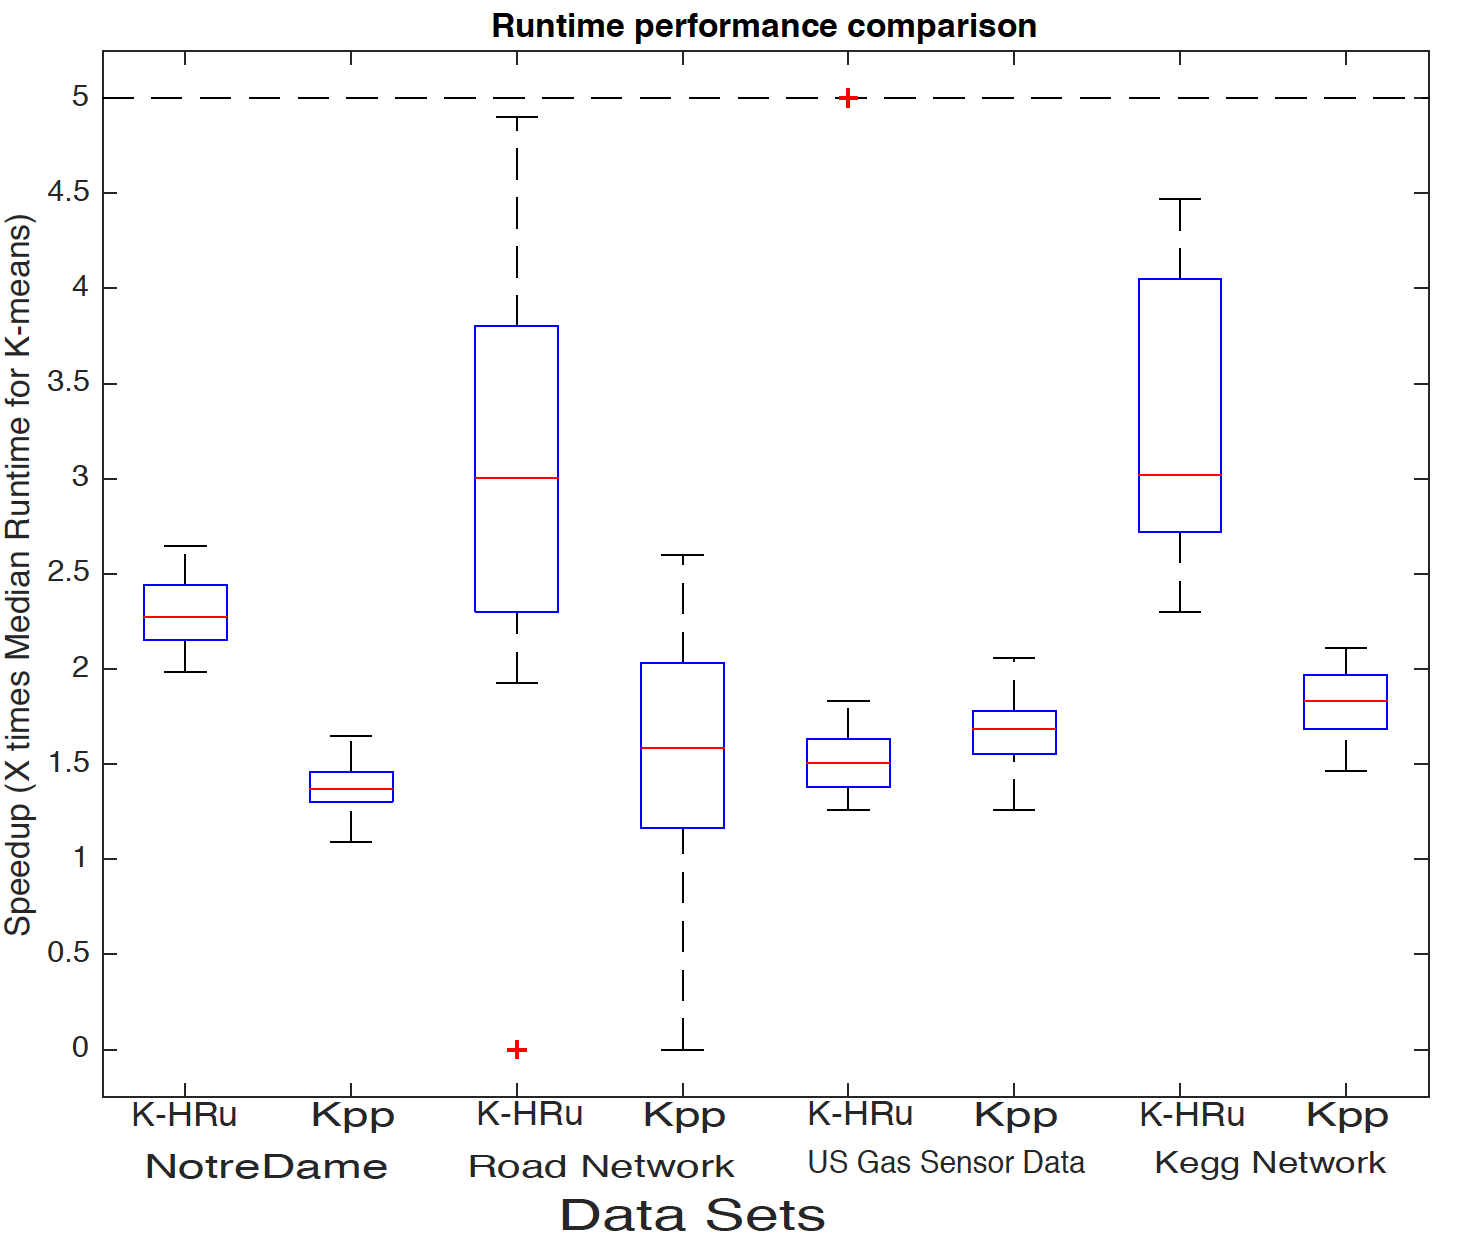
\includegraphics[width=\textwidth]{Chapter-5/figs/kpp+k_cust_speedup_small}
    \caption{Median Speed up, Small Data (k=240)(*K-HRu: K-Means-History Reuse; Kpp: K-Means++)}
    \centering
    \label{fig:box_speedup_small}
\end{figure*}

\begin{figure*}[b!]
    \centering
    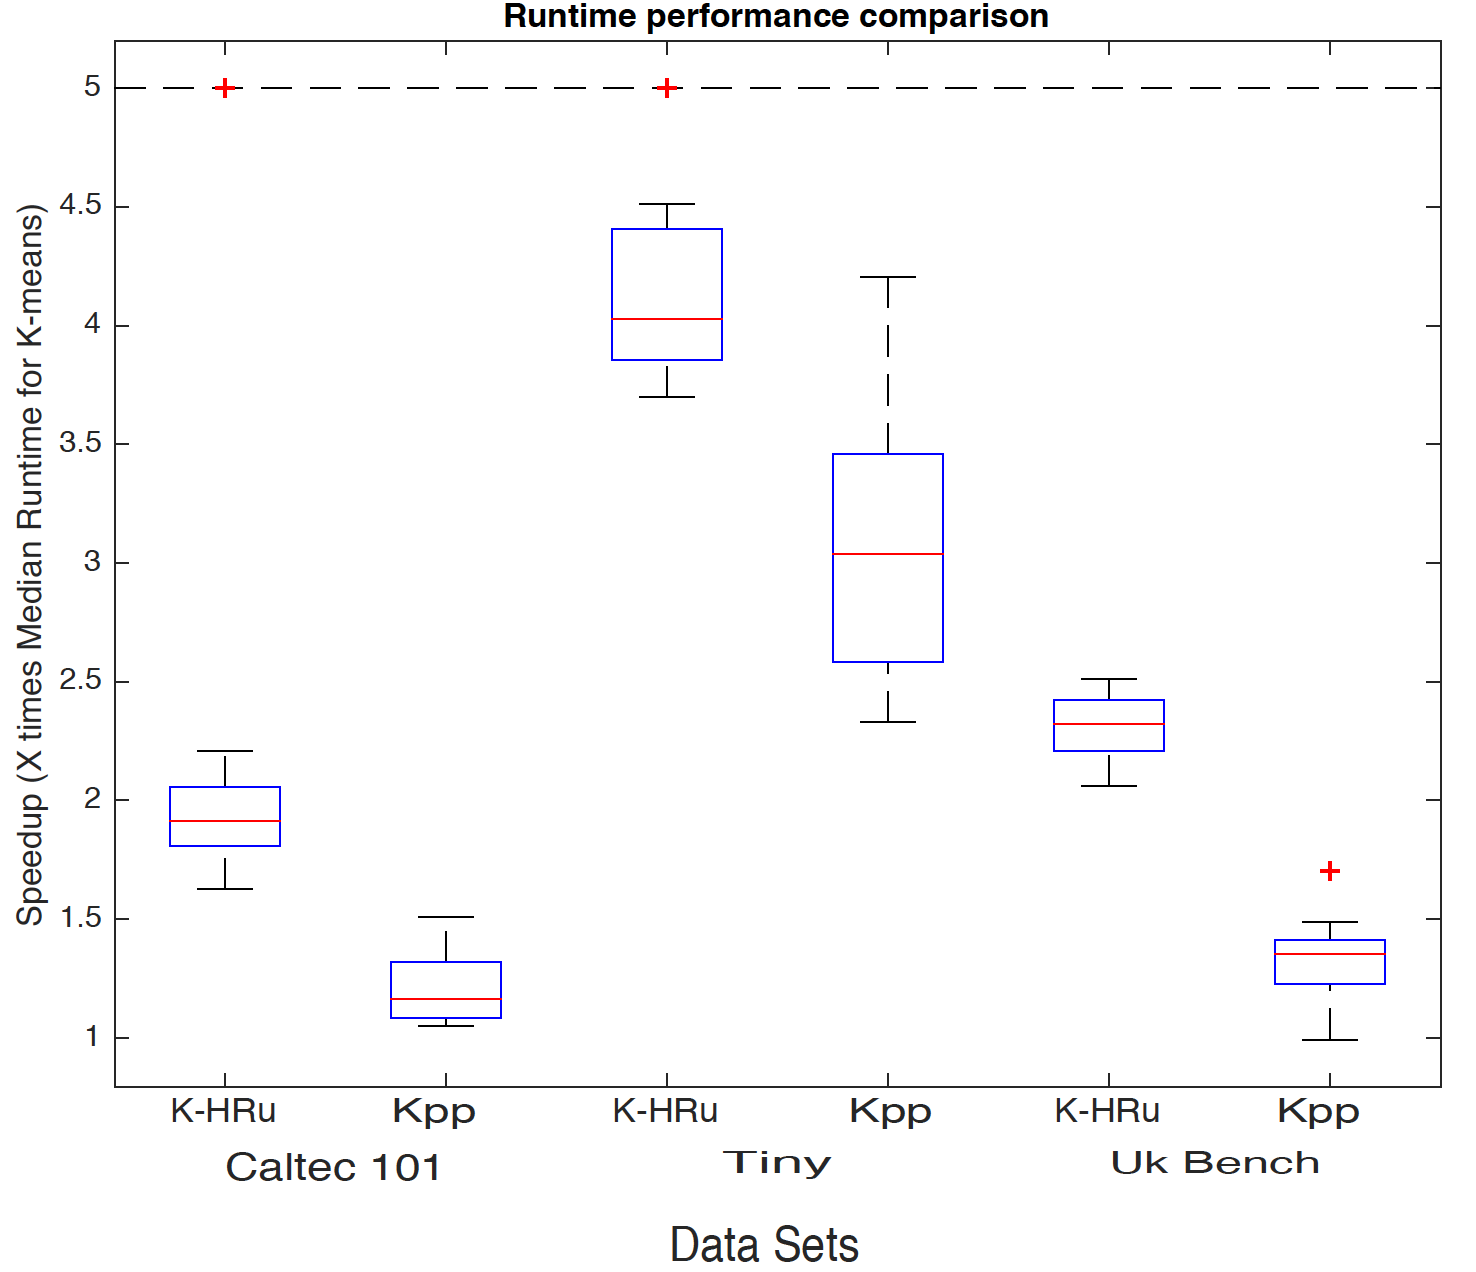
\includegraphics[width=\textwidth]{Chapter-5/figs/kcust+kpp_speedup_large}
    \caption{Median Speed up, Large Data (k=600)(*K-HRu: K-Means-History Reuse; Kpp: K-Means++)}
    \label{fig:box_speedup_large}
\end{figure*}

Another interesting feature seen in the above box plots is the varying degrees of speed up seen for the various segments for same data sets. Looking at the speed up that \textit{K-Means with History Reuse} achieves over the original \textit{K-Means (Lloyd’s algorithm)} we can see that the speed up is generally spread out over a larger range as compared to the performance of the \textit{K-Means++ algorithm} as compared to \textit{Lloyd’s Algorithm}. This thus, brings to fore our above made assumption about the quality of history data set available in terms of the probability of similarity . Our experiments prove our intuitive hypothesis that probabilistically similar data sets will tend to be classed together into similar clusters, thus making them the best history match data sets. The larger variance seen in the box plots above is testament to this. Normalization using \textit{PCA} of data sets, tends to mitigate this to a large extent thus providing us the ability to use history data not along same planes as well and thus providing a consistent speed up, but a better match of normalized data would provide even higher speed ups. We consistently saw that maximum speed ups are seen when the probability of similarity is higher. For segment with high probabilistic similarity we saw speed ups of up to and above \textit{\textbf{100 X}}.
